\documentclass[tikz, border=10pt]{standalone}
\usepackage{pgfplots}
\pgfplotsset{compat=1.18}

\begin{document}
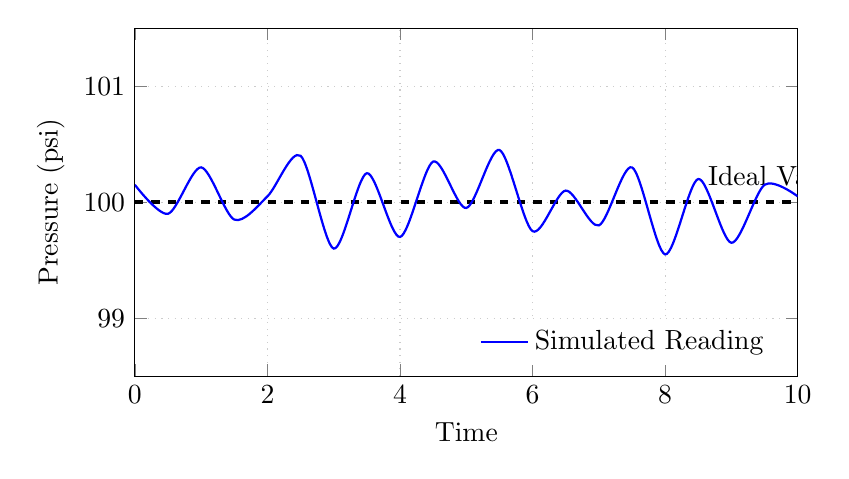
\begin{tikzpicture}
\begin{axis}[
    % Axis Setup
    xlabel={Time},
    ylabel={Pressure (psi)},
    ymin=98.5, ymax=101.5, % Tight Y-limit to visually emphasize the low noise_level
    xmin=0, xmax=10,
    grid=major,
    major grid style={draw=gray!40, dotted}, % Light grid background
    legend pos=south east, % Position legend inside the plot area
    legend style={draw=none}, % Optional: remove box around legend
    width=10cm,
    height=6cm
]

% 1. Ideal Value Line (Dashed, Horizontal)
% The 'forget plot' option ensures this plot is not automatically added to the legend.
\addplot[dashed, black, ultra thick, forget plot] coordinates {(0, 100.0) (10, 100.0)};

% Add a node to label the ideal line explicitly
\node[anchor=south west, black] at (axis cs: 8.5, 100.0) {Ideal Value (100.0 psi)};

% 2. Simulated Reading Line (Solid, Noisy)
% Data points with rapid, random, small fluctuations around 100.
% The 'smooth' option is used to make it look like a continuous, noisy signal.
\addplot[solid, blue, thick, smooth] coordinates {
    (0.0, 100.15) (0.5, 99.90) (1.0, 100.30) (1.5, 99.85) (2.0, 100.05)
    (2.5, 100.40) (3.0, 99.60) (3.5, 100.25) (4.0, 99.70) (4.5, 100.35)
    (5.0, 99.95) (5.5, 100.45) (6.0, 99.75) (6.5, 100.10) (7.0, 99.80)
    (7.5, 100.30) (8.0, 99.55) (8.5, 100.20) (9.0, 99.65) (9.5, 100.15)
    (10.0, 100.05)
};
\addlegendentry{Simulated Reading}

\end{axis}
\end{tikzpicture}
\end{document}